\documentclass{beamer}

%\usetheme{Darmstadt}
%\usefonttheme[onlylarge]{structurebold}
%\setbeamerfont*{frametitle}{size=\normalsize,series=\bfseries}
%\setbeamertemplate{navigation symbols}{}


% Standard packages

\usepackage{graphicx}
\usepackage[english]{babel}
\usepackage[latin1]{inputenc}
\usepackage{times}
\usepackage[T1]{fontenc}
\usepackage{graphicx}


% Setup TikZ

\usepackage{tikz}
\usetikzlibrary{arrows}
\tikzstyle{block}=[draw opacity=0.7,line width=1.4cm]


% Author, Title, etc.

\title
{%
  Exaile Media Player:\\
  An Open Source Introspection....?? %
}

\author
{
  Abhishek Mukherjee \and
  Roy Wellington
}

% The main document

\begin{document}

\begin{frame}
  \titlepage
\end{frame}

\begin{frame}{Outline}
  \tableofcontents
\end{frame}


\section{Introduction}

\subsection{Exaile}

\begin{frame}{Wotsit do?}
  \begin{quote}
    Exaile is a music manager and player for GTK+ written in Python.
  \end{quote}
  \begin{figure}
    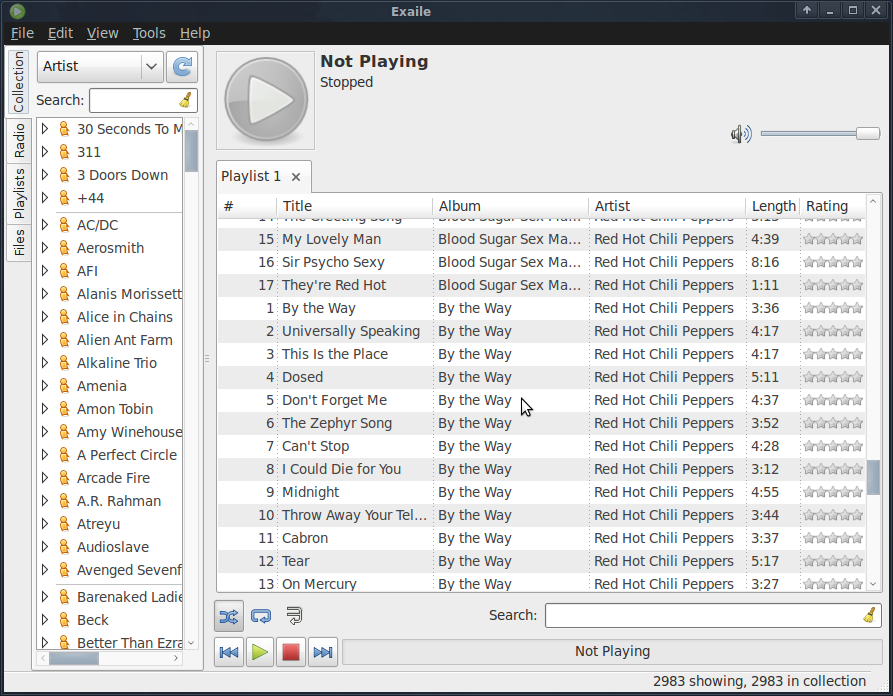
\includegraphics[height=60mm]{images/exaile}
    \caption{The Program}
  \end{figure}
\end{frame}

\begin{frame}{Project Statistics}
  Code statistics for Exaile:
  \begin{itemize}
    \item 23775 lines of Python
    \item $\sim$5000 lines of XML
    \item $\sim$166.5k lines of translations
	\item Counting plugins:
	\begin{itemize}
      \item 22097 lines of Python (plugins)
      \item 4175 lines of XML (plugins)
      \item 2329 lines of C (plugins)
	\end{itemize}
  \end{itemize}
\end{frame}

\section{Feature: Selection randomization}

\begin{frame}{Feature: Selection randomization}
  \begin{itemize}
     \item Exaile originally only allows randomization of an entire playlist
     \item Our change allows a user to randomize a selected part of a playlist.
  \end{itemize}
\end{frame}

\begin{frame}{Why randomize?}
  Many people ask why not just use shuffle.
  \begin{itemize}
    \item Shuffle doesn't allow you to see what's next/previous.
	\item Shuffle doesn't allow you to custom order a subset of the playlist.
  \end{itemize}
\end{frame}

\begin{frame}{The Old Way}
  \begin{itemize}
    \item Select this from the menu:

    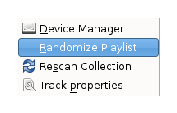
\includegraphics[keepaspectratio]{images/tools-menu}
    \item And the entire playlist is randomized.
	\item What if we only want to randomize a subset of the playlist?
  \end{itemize}
\end{frame}

\begin{frame}{The New Way}
  \begin{itemize}
  \item Select several things in your playlist:
  \item Right click, then use this menu-item:

    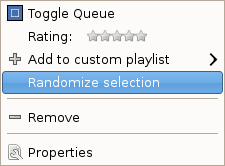
\includegraphics[keepaspectratio]{images/randomize-menu-item}
  \item The selected items are randomized.
  \end{itemize}
\end{frame}

\end{document}
